\documentclass[a4paper]{article}

%% Language and font encodings
\usepackage[english]{babel}
\usepackage[utf8x]{inputenc}
\usepackage[T1]{fontenc}

%% Useful packages
\usepackage{amsmath}
\usepackage{graphicx}
\usepackage[colorinlistoftodos]{todonotes}

\usepackage{url}
\bibliographystyle{plain}

\title{Probability of Unique Fingerprints}
\author{Paige Bateman, Zeke DeSantis, Jackie Preston, Victor Zhang}

\begin{document}
\maketitle

\tableofcontents

\section{Introduction}

This paper describes the model we created to find the probability that every fingerprint is unique. Fingerprints are small ridges on the skin of the palms and fingers which potentially help with gripping, touch sensitivity, and more durable skin, although their true purpose is still disputed. Although fingerprints have the potential to be completely unique, the fingerprints of people follow many similar patterns and have similar details.  We model fingerprints by examining different minutiae points on the finger and then compare it to every other fingerprint in the database that we created. These minutiae points have a Gamma distribution. The results are modeled in a ROC curve. 

\subsection{Current Techniques}
Fingerprints can be classified based on large scale structures, small scale structures, or by computer imaging algorithms. Comparing the structures attempts to teach computers to look at the fingerprint like a person would look at it to make comparisons. Using imaging algorithms makes use of the special techniques available to computers to compare the images instead of trying to compare the prints from which the images came.

To compare fingerprints based on large scale ridge structure the prints first need to be classified as one of five types of ridge structure: arches, tented arches, whorls, and left and right loops (see figure \ref{fig:structures}).
\begin{figure}
\centering
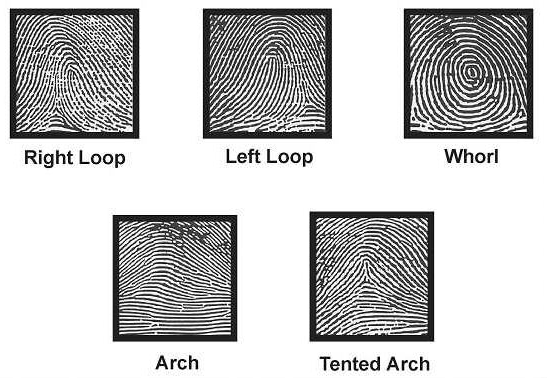
\includegraphics[width=8cm]{Structure_Types.PNG}
\caption{Types of fingerprint structures.}
\label{fig:structures}
\end{figure}
Each structure has its own set of parameters that can be used to define a print of that type. These parameters are points, lengths, and angles that can be used to compare prints of the same structure type. \cite[219-221]{umap} An example of an arch print and the dimensions associated with it can be seen in figure \ref{fig:arch} and figure \ref{fig:archdim}.
\begin{figure}
\centering
\begin{minipage}[b]{0.4\textwidth}
    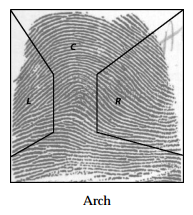
\includegraphics[width=5cm]{Arch.PNG}
    \caption{Sample arch structure}
    \label{fig:arch}
  \end{minipage}
  \hfill
  \begin{minipage}[b]{0.4\textwidth}
    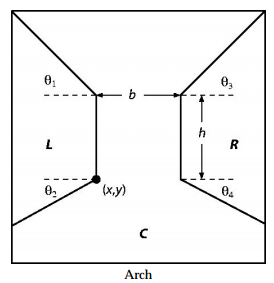
\includegraphics[width=5cm]{Arch_Dimensions.PNG}
    \caption{Dimensions used to specify arch structure}
    \label{fig:archdim}
  \end{minipage}
\end{figure}

Small scale structures, called minutiae, come in three types: dots, bifurcations, and terminations \cite[217-218]{umap} (see figure \ref{fig:minutiaetype}).
\begin{figure}
\centering
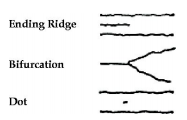
\includegraphics[width=8cm]{Minutiae_Types.PNG}
\caption{Types of minutiae}
\label{fig:minutiaetype}
\end{figure}
Minutiae are specified on a print by location, direction of the ridge they are a part of, and if the matching software is advanced enough it will also include the type of minutiae. Prints are matched using minutiae by first finding all the minutiae in each print and then comparing the vector fields of the two prints as shown in figure \ref{fig:minutiaematch}.
\begin{figure}
\centering
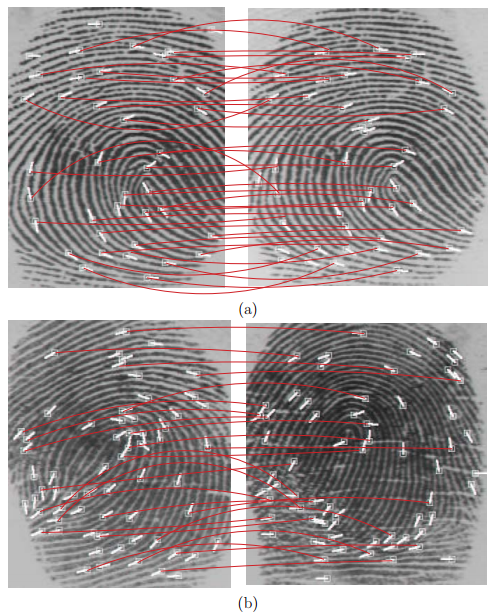
\includegraphics[width=8cm]{Minutiae_Matching.PNG}
\caption{An example of matching fingerprints by minutiae. (a) shows the same finger with 36 of 39 "true" correspondences and (b) shows different fingers with 25 of 64 "false" correspondences.}
\label{fig:minutiaematch}
\end{figure}
Results are normalized so that the number of minutiae per fingerprint does not affect the outcome. \cite{prabhakar}

Another way to digitalize prints is to separate the image of the fingerprint into segments and calculate the grayscale intensity of each segment. Each print in the matching database is stored as a template that includes rotations of the grayscale image to within forty-five degrees either direction. The rotations are stored to account for any difference in orientation between the template and the input print.  When matching prints the Euclidean distance between the vectors for the two prints is calculated. One downfall of this method is that a reference point is necessary to define the middle from which the segments originate. If the images to compare differ in quality then even if they are of the same print the reference point may not be the same and thus the intensity vectors would not be the same and the prints would be deemed different. \cite{prabhakar}
\begin{figure}
\centering
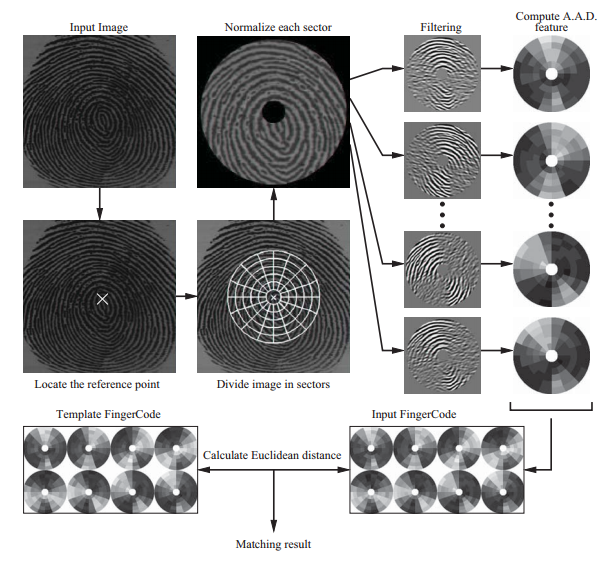
\includegraphics[width=8cm]{Algorithm.PNG}
\caption{Diagram of fingerprint authentication}
\label{fig:algorithm}
\end{figure}

\subsection{The Gamma Distribution}

For a random variable $X$, the standard gamma distribution is defined as the distribution, with shape parameter $k \in (0, \infty)$, of the probability density function $$f(x) = \frac{1}{\Gamma(k)} x^{k-1} e^{-x}$$ The function $\Gamma(k)$ is the gamma function and is defined as $$\Gamma(k) = \int_0^\infty x^{k-1} e^{-x} dx$$
In our model, the minutiae points have a gamma distribution \cite{gammadist}.

\subsection{The ROC Curve}
A Receiver Operating Characteristic curve (ROC curve) plots the true positive rate against the false positive rate. This is done by measuring the two rates at different levels of strictness. The plot then demonstrates how many correct and how many incorrect matches are obtained by lowering the stictness of the test. A very bad test will be along the y=x line meaning that the rate of true positive and the rate of false positives are equal. This means that your test is no better than random guessing. A perfect test will be a right angle with zero percent false positives and one hundred percent true positives. The accuracy of a test is determined by the area under the curve. An area of 0.5 corresponds to random guessing and an area of 1 corresponds to a perfect test. The traditional system for areas in between is: 0.9-1 is excellent, 0.8-0.9 is good, 0.7-0.8 is fair, 0.6-0.7 is poor, and 0.5-0.6 is failure. \cite{ROCnotes}

\section{Model}

The distribution of minutiae on the fingerprints of a population of people can best be modeled as a gamma distribution centered around the core of the fingerprint. For our model the gamma distribution has a shape parameter of 0.193 and a scale parameter of 5.91mm.

Our model was created as a simulation. To begin, a certain number of people's fingerprint details are added to the dataset. A test picked a random record from the dataset and is matched on each minutiae point using the k-nearest-neighbor (knn) algorithm. The parameter $k$ in knn is set to $1$ in the test, since $k > 1$ will not give much information for identifying one record as a mean of some other records. Then each minutiae point is matched to its particular group. The person whose fingerprint matches the minutiae points found most frequently is the predicted person.   For example, say there are three minutiae points that the model is looking at and there are three fingerprints in the dataset. If the first minutiae is matched with person 1 and the second and third minutiae points are matched with person 2, the algorithm will say that the matching person is person 2. For our model, the number of fingerprints in the dataset can be changed to obtain different results, as can the standard deviation.

\section{Analysis}
The goal of the model is to make the false positive rate as small as possible in order to conclude that the fingerprint is being matched properly. From our model, we can see that different numbers of fingerprints and different standard deviations have a large effect on the ROC curve that we produce. To begin we tested 30 fingerprints with a standard deviation of 0.01. The ROC curve produced with these numbers is shown in figure \ref{fig:ROC1}. We conclude that the false positive rate for these numbers is 0.275. This is too large for us to make any positive conclusions about the results of the fingerprint matching. 

By changing the standard deviation to 0.005 while keeping the number of fingerprints tested the same, as shown in figure \ref{fig:ROC2}, we conclude that the false positive rate is 0.035. This number is much smaller and lets us conclude that the fingerprint that is tested actually matches the person it is supposed to. By decreasing the standard deviation even further to $2e^{-4}$, as shown in figure \ref{fig:ROC3}, the false positive rate decreases to 0, allowing us to conclude that we have a perfect match.

We then increase the number of fingerprints tested to 50 with a standard deviation of 0.005. The ROC curve shown in figure \ref{fig:ROC4} shows the false positive rate to be 0.035. This is the same as the false positive rate with 30 fingerprints and the same standard deviation. The issue arises when we try to test 100 fingerprints. As shown in figure \ref{fig:ROC5}, when we increase to 100 fingerprints and a standard deviation of 0.005, the false positive rate jumps to 0.165. This rate is too high for us to make a positive conclusion. 


\begin{figure}
\centering
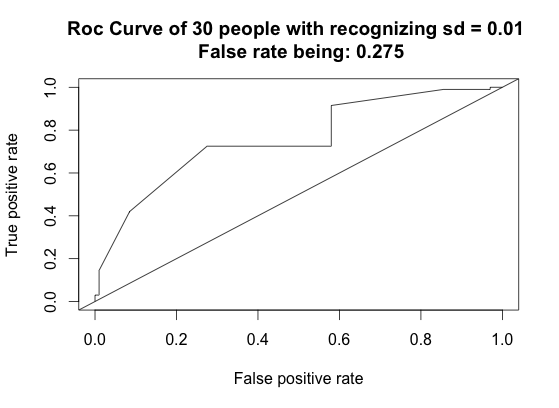
\includegraphics[width=13cm]{Roc1.png}
\caption{ROC curve for 30 fingerprints with standard deviation 0.01}
\label{fig:ROC1}
\end{figure}

\begin{figure}
\centering
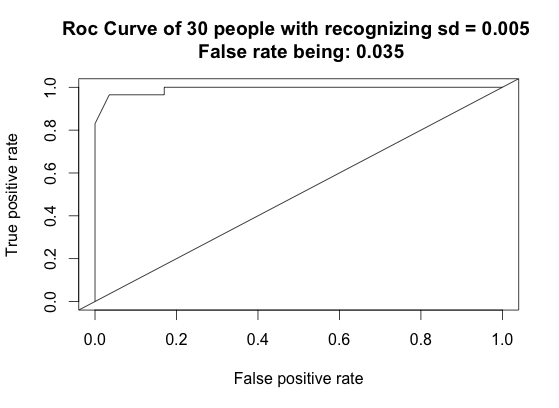
\includegraphics[width=13cm]{Roc2.png}
\caption{ROC curve for 30 fingerprints with standard deviation 0.005}
\label{fig:ROC2}
\end{figure}

\begin{figure}
\centering
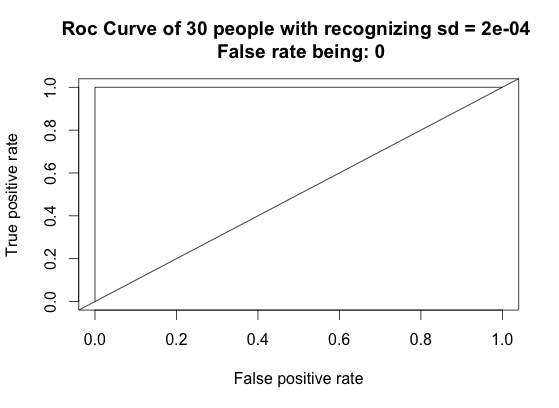
\includegraphics[width=13cm]{Roc3.png}
\caption{ROC curve for 30 fingerprints with standard deviation $2e^{-4}$}
\label{fig:ROC3}
\end{figure}

\begin{figure}
\centering
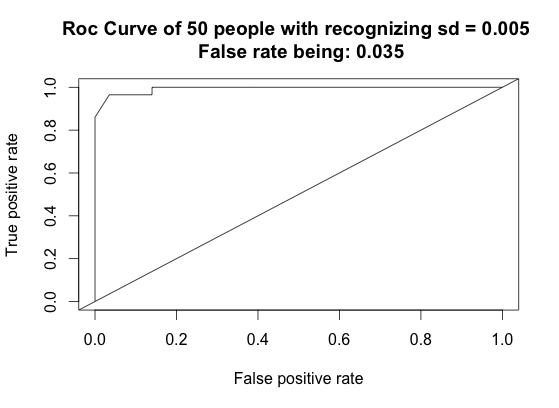
\includegraphics[width=13cm]{Roc4.png}
\caption{ROC curve for 50 fingerprints with standard deviation 0.005}
\label{fig:ROC4}
\end{figure}

\begin{figure}
\centering
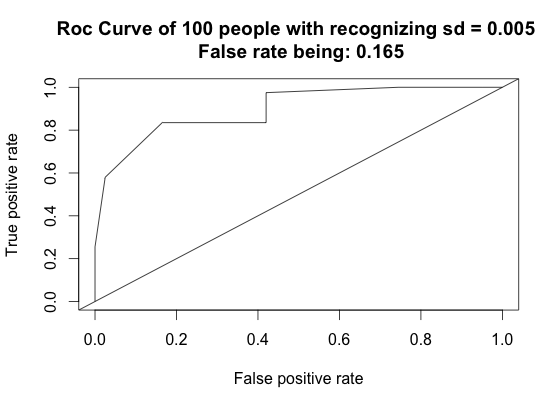
\includegraphics[width=13cm]{Roc5.png}
\caption{ROC curve for 100 fingerprints with standard deviation 0.005}
\label{fig:ROC5}
\end{figure}

\newpage
\section{Conclusions}
We found that the probability of the fingerprint being tested being unique is dependent upon how many people are in our database and the standard deviation. In general, the best results came from a standard deviation of $2e^{-4}$. This standard deviation is not very realistic, so the best and most realistic results came from a standard deviation of 0.005. In our model, the odds of misidentification by fingerprint evidence changes depending on the number of fingerprints tested and the standard deviation. The odds of misidentification by DNA evidence are not well publicized. In an article from 2008, the FBI's rate of DNA misidentification was said to be 1 in 113 billion, but the author of the paper found it to be more like 1 in 13 billion \cite{DNA}. 

\newpage
\bibliography{sources.bib}

\end{document}